\chapter{Conclusion}

Although improvements are still needed, several statements can be made regarding the data collected which helps the understanding of the solar thermal power generation system and changes that can improve the experiment.
    
As seen in Figure \ref{fig:trend}, the output follows a relatively linear relationship as the temperature increases. At temperatures less than 110\degree C, the engine was not running. Any output data seen in this range is due to manually spinning the flywheel to jump-start the engine. In order to better understand the analysis of the data, the following is an interpretation using a line fit to the data:

By ignoring engine jump-start output data and outputs that are less than the maximum and fitting a trend line, there are a number of trends that can be noticed. In the range from about 110-160\degree C, output increases exponentially and then the increasing rate decreases. Near the lower end of this range an increase in temperature gives a much greater output, while near the upper end of this range an increase in temperature results in a decreasing return in output.

\begin{figure}[H]
    \centering
    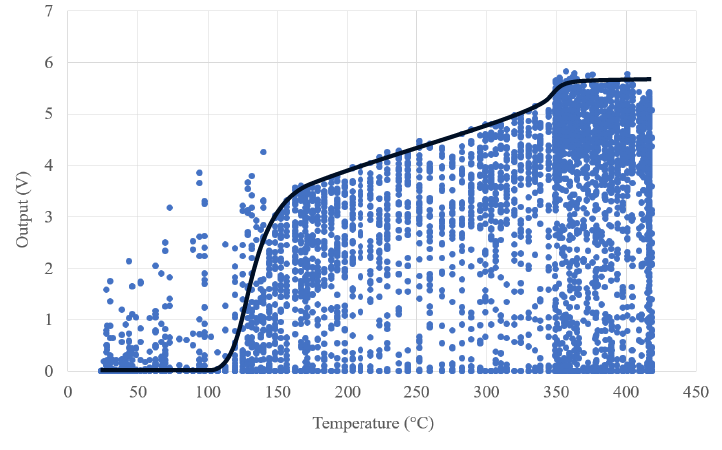
\includegraphics[width=\textwidth]{diagrams/data3trend}
    \caption[Data with trend line interpretation]{Output voltage versus Stirling engine temperature with manual trend line applied.}
    \label{fig:trend}
\end{figure}

From 160-350\degree C, the output follows a very close linear function. This is interesting because not all of the data show the same relationship. Above 350\degree C, the output begins to reach a rough maximum of about 5.5V. Again, the density of this range can be explained when referring back to Figure \ref{fig:timedata}.

To conclude, the operating temperature of this Stirling engine is most efficient given a variable temperature at 160\degree C. At slightly lower temperatures, the output is much less. At slightly higher temperatures, the output gained does not make the extra fuel worthwhile due to its small-slope linear relationship. Stirling engine-based solar power could be a viable form of alternative energy which utilizes sunlight.

\section{Sources of Uncertainty}
    
    The issues to be addressed relate to the output from the generator and several other factors. The generator which produced the voltage output was not used as designed since it is actually a brushless D.C. motor running in reverse, therefore it did not run with optimal efficiency. In addition, the Stirling engine and its cycle is imperfect and inconsistent. A smaller system also means there is more uncertainty in the results.

\section{Future Work}

    As this experiment was created from the ground-up, progress has been made to make a working small-scale prototype for a solar thermal Stirling engine. Once the current issues are resolved and proper data taken, the viability of this system can be further tested. This includes scaling, production cost, and optimization based on data collected. It would also be beneficial to test and improve the engine's efficiency of this system and compare it with modern solar cells.